% The Transformer, from Tokens to Text -- a 20-frame tutorial.
% Build from this directory:   latexmk -pdf transformer_tutorial.tex
% Needs: beamer + metropolis theme, tikz, pgfplots, listings (all in TeX Live).
% Frames 9 and 19 read data written by ../make_figures.py into generated/;
% frames 17-18 pull their listings directly from ../model.py and ../train.py.
\documentclass[aspectratio=169,10pt]{beamer}

\usetheme[numbering=fraction,progressbar=frametitle,block=fill]{metropolis}
\geometry{papersize={192mm,108mm}}
\usefonttheme[onlymath]{serif}
\usepackage{amsmath,amssymb,bm,booktabs,array}
\usepackage{tikz,pgfplots,listings}
\pgfplotsset{compat=1.17}
\usetikzlibrary{arrows.meta,positioning,calc,fit,backgrounds,decorations.pathreplacing,matrix}

% ---------------------------------------------------------------- colours
% One colour per stage, used consistently in every diagram.
\definecolor{cInk}{HTML}{22303C}
\definecolor{cTok}{HTML}{5B6770}   % tokens / ids
\definecolor{cEmb}{HTML}{2F6DB5}   % embeddings
\definecolor{cAtt}{HTML}{D9822B}   % attention
\definecolor{cFfn}{HTML}{2E8B57}   % feed-forward
\definecolor{cNrm}{HTML}{8C7A2B}   % normalisation
\definecolor{cOut}{HTML}{7B4FA6}   % output / sampling
\definecolor{cBad}{HTML}{B03A3A}
\setbeamercolor{normal text}{fg=cInk,bg=white}
\setbeamercolor{frametitle}{bg=cInk,fg=white}
\setbeamercolor{progress bar}{fg=cAtt,bg=cAtt!25}
\setbeamercolor{alerted text}{fg=cAtt}
\setbeamercolor{block title}{bg=cEmb!14,fg=cInk}
\setbeamercolor{block body}{bg=cEmb!5}
\setbeamerfont{block title}{series=\bfseries,size=\small}
\setbeamertemplate{itemize item}{\color{cAtt}\rule[0.25ex]{0.9ex}{0.9ex}}
\setbeamertemplate{itemize subitem}{\color{cTok}--}
\setlength{\leftmargini}{1.1em}

% ---------------------------------------------------------------- macros
\newcommand{\R}{\mathbb{R}}
\DeclareMathOperator{\softmax}{softmax}
\DeclareMathOperator{\LN}{LN}
\DeclareMathOperator{\MHA}{MHA}
\DeclareMathOperator{\FFN}{FFN}
\DeclareMathOperator{\Attn}{Attn}
\DeclareMathOperator{\GELU}{GELU}
\newcommand{\T}{\top}
\renewcommand{\cite}[1]{{\scriptsize\color{cTok}[#1]}}
\newcommand{\vsp}{\textvisiblespace}
\newcommand{\key}[1]{\textbf{\color{cAtt}#1}}

\tikzset{
  >={Stealth[length=5pt]},
  stage/.style={draw=#1,fill=#1!12,rounded corners=2pt,line width=0.7pt,
                minimum height=7.5mm,inner xsep=5pt,font=\small,align=center},
  stage/.default=cTok,
  flow/.style={->,line width=0.7pt,draw=cInk!80},
  note/.style={font=\scriptsize,text=cTok,align=center},
  tokbox/.style={draw=cTok,fill=cTok!10,rounded corners=1.5pt,font=\ttfamily\small,
                 minimum height=5.5mm,inner xsep=3pt,outer sep=0pt},
  cell/.style={minimum size=5mm,inner sep=0pt,font=\scriptsize},
}

\lstdefinestyle{py}{
  language=Python,basicstyle=\ttfamily\fontsize{6.1}{7.4}\selectfont,
  keywordstyle=\color{cEmb}\bfseries,commentstyle=\color{cFfn!85!black}\itshape,
  stringstyle=\color{cAtt!85!black},showstringspaces=false,columns=fullflexible,
  keepspaces=true,frame=none,backgroundcolor=\color{cInk!4},
  xleftmargin=3pt,xrightmargin=3pt,aboveskip=2pt,belowskip=2pt,
  literate={-}{{-}}1,
}

\title{The Transformer, from Tokens to Text}
\subtitle{How a decoder-only, dense LLM works: the math, the diagrams, and runnable code}
\date{A 20-slide tutorial \textbullet{} companion code: \texttt{tokenizer.py}, \texttt{model.py},
      \texttt{train.py}, \texttt{walkthrough.py}}

\newcommand{\resSteps}{3{,}000}
\newcommand{\resMinutes}{16}
\newcommand{\resInit}{6.26}
\newcommand{\resTrain}{2.60}
\newcommand{\resVal}{3.03}
\newcommand{\resBestStep}{2{,}750}
\newcommand{\resPpl}{21}

\begin{document}

% ======================================================================= 1
\maketitle
\addtocounter{framenumber}{1}

% ======================================================================= 2
\begin{frame}{The job: predict the next token}
\begin{columns}[T,onlytextwidth]
\column{0.50\textwidth}
A language model assigns a probability to a token sequence. The chain rule
turns that into a sequence of next-token predictions:
\[
  p(x_1,\dots,x_T)\;=\;\prod_{t=1}^{T} p_\theta\bigl(x_t \mid x_1,\dots,x_{t-1}\bigr).
\]
\column{0.46\textwidth}
\begin{itemize}\small
  \item \key{Decoder-only}: one stack; each position sees only tokens to its left (GPT family \cite{2,3}).
  \item \key{Dense}: every parameter is used for every token (no expert routing, as in MoE models).
\end{itemize}
\end{columns}
\vspace{2mm}
\centering
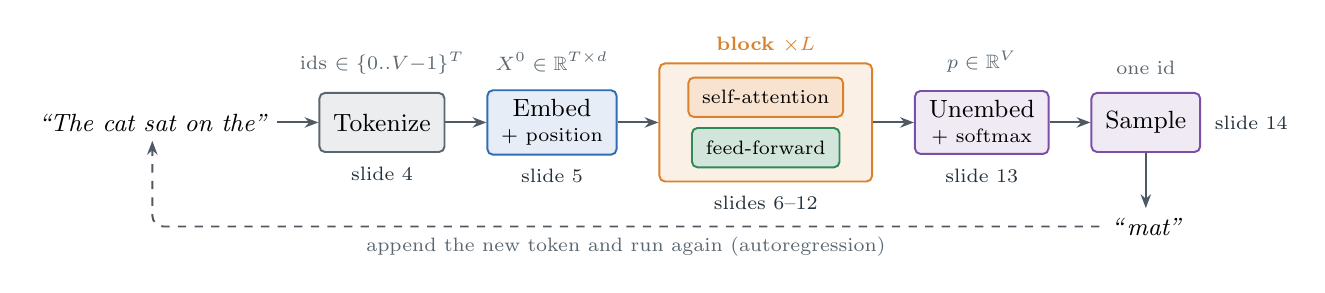
\begin{tikzpicture}[node distance=5.2mm]
  \node[font=\small\itshape] (txt) {``The cat sat on the''};
  \node[stage=cTok,right=of txt] (tok) {Tokenize};
  \node[stage=cEmb,right=of tok] (emb) {Embed\\[-2pt]{\scriptsize + position}};
  \node[stage=cAtt,right=of emb,minimum height=15mm,minimum width=27mm] (blk) {};
  \node[stage=cAtt,fill=cAtt!22,minimum height=5mm,font=\scriptsize] at ($(blk.center)+(0,3.2mm)$) (att) {self-attention};
  \node[stage=cFfn,fill=cFfn!22,minimum height=5mm,font=\scriptsize] at ($(blk.center)+(0,-3.2mm)$) (ffn) {feed-forward};
  \node[font=\scriptsize\bfseries,text=cAtt,anchor=south] at (blk.north) {block $\times L$};
  \node[stage=cOut,right=of blk] (out) {Unembed\\[-2pt]{\scriptsize + softmax}};
  \node[stage=cOut,right=of out] (smp) {Sample};
  \node[font=\small\itshape,below=7mm of smp] (nxt) {``\,mat''};
  \draw[flow] (txt)--(tok); \draw[flow] (tok)--(emb); \draw[flow] (emb)--(blk);
  \draw[flow] (blk)--(out); \draw[flow] (out)--(smp); \draw[flow] (smp)--(nxt);
  \draw[flow,dashed,rounded corners=4pt] (nxt.west) -| node[pos=0.25,below,note]{append the new token and run again (autoregression)} (txt.south);
  % what flows on each wire
  \node[note,above=1mm of tok] {ids $\in\{0..V{-}1\}^T$};
  \node[note,above=1mm of emb] {$X^0\in\R^{T\times d}$};
  \node[note,above=1mm of out] {$p\in\R^{V}$};
  \node[note,above=1mm of smp] {one id};
  % roadmap
  \node[note,below=0.5mm of tok,text=cInk] {slide 4};
  \node[note,below=0.5mm of emb,text=cInk] {slide 5};
  \node[note,below=0.5mm of blk,text=cInk] {slides 6--12};
  \node[note,below=0.5mm of out,text=cInk] {slide 13};
  \node[note,right=0.5mm of smp,text=cInk] {slide 14};
\end{tikzpicture}

\vspace{1mm}
{\small Everything between ``Tokenize'' and ``Sample'' is one differentiable function $f_\theta$;
training (slides 15--16) adjusts $\theta$ so the true next token gets high probability.}
\end{frame}

% ======================================================================= 3
\begin{frame}{Notation: six numbers define the model}
\begin{columns}[T,onlytextwidth]
\column{0.57\textwidth}
\small
\renewcommand{\arraystretch}{1.18}
\begin{tabular}{@{}clrr@{}}
\toprule
 & meaning & \textbf{this tutorial} & GPT-2 small \cite{3}\\
\midrule
$V$ & vocabulary size & 512 & 50{,}257\\
$T_{\max}$ & context window (tokens) & 128 & 1{,}024\\
$d$ & model width & 128 & 768\\
$h$ & attention heads & 4 & 12\\
$d_k$ & width of one head, $d/h$ & 32 & 64\\
$L$ & number of blocks & 4 & 12\\
\midrule
 & parameters & 875{,}264 & 124\,M\\
\bottomrule
\end{tabular}

\vspace{2.5mm}
Same architecture, same equations: only these six numbers change between a laptop
model and a production one.
\column{0.39\textwidth}
\begin{block}{Conventions}
\small
\begin{itemize}
  \item A sequence is a matrix $X\in\R^{T\times d}$: \textbf{one row per token}.
  \item Vectors are rows, so a linear layer is $xW$ with $W\in\R{}^{d_\text{in}\times d_\text{out}}$.
  \item $X^{\ell}$ is the matrix after block $\ell$; $X^{0}$ is the embedding.
  \item $x_t$ is row $t$: ``what the model knows at position $t$''.
\end{itemize}
\end{block}
\vspace{-1mm}
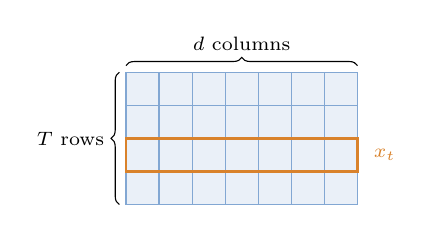
\begin{tikzpicture}[x=4.2mm,y=4.2mm]
  \foreach \r in {0,...,3} \foreach \c in {0,...,6}
     \draw[cEmb!60,fill=cEmb!10] (\c,-\r) rectangle ++(1,-1);
  \draw[cAtt,line width=1pt] (0,-2) rectangle (7,-3);
  \draw[decorate,decoration={brace,amplitude=3pt}] (0,0.2)--(7,0.2) node[midway,above=2pt,font=\scriptsize]{$d$ columns};
  \draw[decorate,decoration={brace,amplitude=3pt,mirror}] (-0.2,0)--(-0.2,-4) node[midway,left=2pt,font=\scriptsize]{$T$ rows};
  \node[font=\scriptsize,text=cAtt,anchor=west] at (7.2,-2.5) {$x_t$};
\end{tikzpicture}
\end{columns}
\end{frame}

% ======================================================================= 4
\begin{frame}{Stage 1 \textbullet{} Tokenization: text becomes integers}
\begin{columns}[T,onlytextwidth]
\column{0.47\textwidth}
\small
A network needs numbers. Which units of text get a number?
\begin{itemize}
  \item \textbf{Characters}: tiny vocabulary, very long sequences.
  \item \textbf{Words}: short sequences, but unseen words are unrepresentable.
  \item \key{Subwords}: common words are one token, rare words split into pieces.
\end{itemize}
\begin{block}{Byte-pair encoding (BPE) \cite{4}}
\begin{enumerate}\small
  \item Start with one token per byte (256 tokens).
  \item Count every adjacent pair of tokens in the corpus.
  \item Merge the most frequent pair into a new token.
  \item Repeat 2--3 until the vocabulary has $V$ entries.
\end{enumerate}
\end{block}
To encode new text, replay the merges in the order learned. Decoding is concatenation, so
tokenization is lossless.
\column{0.50\textwidth}
\small
\textbf{Toy corpus} (word:count)\ \ {\ttfamily\footnotesize low:5\ lower:2\ newest:6\ widest:3}

\vspace{1mm}
{\footnotesize
\begin{tabular}{@{}cllr@{}}
\toprule
merge & pair & new token (id) & count\\
\midrule
1 & \texttt{e + s}   & \texttt{es} (256)   & 9\\
2 & \texttt{es + t}  & \texttt{est} (257)  & 9\\
3 & \texttt{l + o}   & \texttt{lo} (258)   & 7\\
4 & \texttt{lo + w}  & \texttt{low} (259)  & 7\\
\bottomrule
\end{tabular}}

\vspace{1mm}
\texttt{lowest} never occurs in the corpus, yet encodes as two known pieces:

\vspace{1mm}
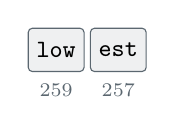
\begin{tikzpicture}[node distance=0.8mm]
  \node[tokbox] (a) {low}; \node[tokbox,right=of a] (b) {est};
  \node[note,below=0.3mm of a] {259}; \node[note,below=0.3mm of b] {257};
\end{tikzpicture}

\vspace{1.5mm}
\textbf{Real example}: our $V{=}512$ tokenizer trained on Shakespeare

\vspace{1mm}
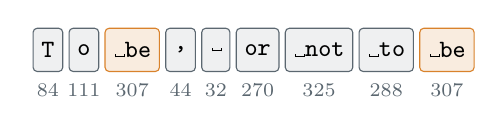
\begin{tikzpicture}[node distance=0.8mm]
  \node[tokbox] (t1) {T};
  \node[tokbox,right=of t1] (t2) {o};
  \node[tokbox,right=of t2,draw=cAtt,fill=cAtt!15] (t3) {\vsp be};
  \node[tokbox,right=of t3] (t4) {,};
  \node[tokbox,right=of t4] (t5) {\vsp};
  \node[tokbox,right=of t5] (t6) {or};
  \node[tokbox,right=of t6] (t7) {\vsp not};
  \node[tokbox,right=of t7] (t8) {\vsp to};
  \node[tokbox,right=of t8,draw=cAtt,fill=cAtt!15] (t9) {\vsp be};
  \foreach \n/\i in {t1/84,t2/111,t3/307,t4/44,t5/32,t6/270,t7/325,t8/288,t9/307}
    \node[note,below=0.3mm of \n] {\i};
\end{tikzpicture}

\vspace{0.5mm}
{\footnotesize 19 characters $\to$ 9 tokens; both \texttt{\vsp be} map to id 307.
Corpus average: 2.00 characters per token.}
\end{columns}
\end{frame}

% ======================================================================= 5
\begin{frame}{Stage 2 \textbullet{} Embedding: integers become vectors}
\begin{columns}[T,onlytextwidth]
\column{0.50\textwidth}
\small
An id is just a name; id 307 is not ``bigger'' than id 44. Give every token a
\textbf{learned vector} instead:
\[
  x^0_t \;=\; \underbrace{E[x_t]}_{\text{what}} \;+\; \underbrace{P[t]}_{\text{where}},
  \qquad E\in\R^{V\times d},\;\; P\in\R^{T_{\max}\times d}.
\]
\begin{itemize}
  \item $E[x_t]$ is \textbf{row $x_t$ of a table}. Equivalently
        $\operatorname{onehot}(x_t)\,E$: a linear layer applied to a one-hot vector.
  \item Training moves tokens used in similar contexts toward similar vectors.
  \item \key{Why $P$?} Attention (next slides) treats its input as a \emph{set}: without
        positions, ``dog bites man'' and ``man bites dog'' look identical.
  \item We learn $P$ like GPT-2 \cite{3}. The original paper used fixed sinusoids \cite{1};
        many recent models rotate queries and keys instead (RoPE \cite{17}).
\end{itemize}
\column{0.47\textwidth}
\centering
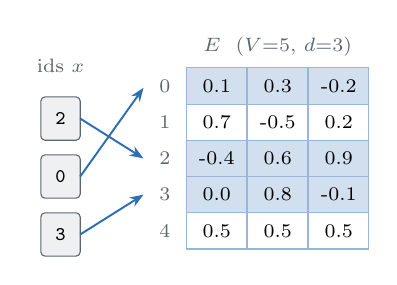
\begin{tikzpicture}[x=6.2mm,y=4.6mm,font=\scriptsize]
  % ids
  \foreach \i/\v in {0/2,1/0,2/3} \node[tokbox,minimum width=5mm,font=\ttfamily\scriptsize] (id\i) at (-3.2,-\i*1.6-0.9) {\v};
  \node[note,above] at (-3.2,0.1) {ids $x$};
  % table E
  \foreach \r/\a/\b/\c in {0/0.1/0.3/-0.2,1/0.7/-0.5/0.2,2/-0.4/0.6/0.9,3/0.0/0.8/-0.1,4/0.5/0.5/0.5}{
    \foreach \cc/\val in {0/\a,1/\b,2/\c}
      \node[cell,draw=cEmb!50,minimum width=7.6mm,minimum height=4.6mm] (e\r\cc) at (\cc*1.25,-\r) {\val};
    \node[note,anchor=east] at (-0.75,-\r) {\r};
  }
  \node[note,above] at (1.25,0.55) {$E$ \ ($V{=}5$, $d{=}3$)};
  \begin{scope}[on background layer]
    \foreach \r in {2,0,3} \fill[cEmb!22] (-0.62,-\r+0.5) rectangle (3.12,-\r-0.5);
  \end{scope}
  \draw[flow,cEmb] (id0.east) -- (-1.5,-2);
  \draw[flow,cEmb] (id1.east) -- (-1.5,-0.05);
  \draw[flow,cEmb] (id2.east) -- (-1.5,-3);
\end{tikzpicture}

\vspace{1mm}
{\scriptsize\setlength{\arraycolsep}{3pt}
\[
\underbrace{\begin{bmatrix}-0.4&0.6&0.9\\0.1&0.3&-0.2\\0.0&0.8&-0.1\end{bmatrix}}_{E[x]}
+\underbrace{\begin{bmatrix}0.0&0.1&0.0\\0.1&0.0&0.1\\0.2&-0.1&0.0\end{bmatrix}}_{P}
=\underbrace{\begin{bmatrix}-0.4&0.7&0.9\\0.2&0.3&-0.1\\0.2&0.7&-0.1\end{bmatrix}}_{X^0}
\]}
\end{columns}
\end{frame}

% ======================================================================= 6
\begin{frame}{Stage 3 \textbullet{} Self-attention: the idea}
\small
The embedding of ``the'' is the same in every sentence. To predict what follows, position $t$
must \textbf{gather information from earlier positions}. Attention is a soft, learnable lookup \cite{1,5}:

\vspace{1mm}
\centering
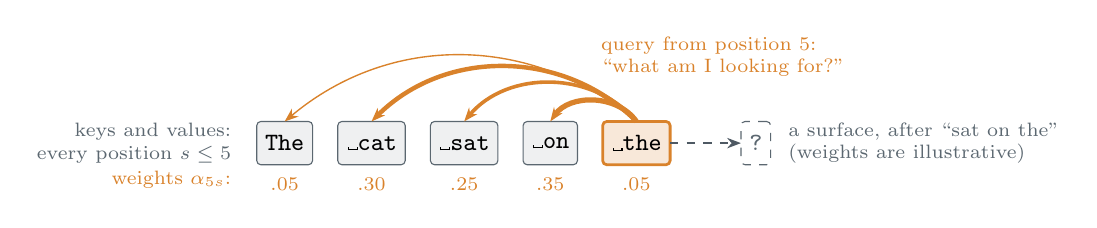
\begin{tikzpicture}[node distance=3.2mm]
  \node[tokbox] (w1) {The};
  \node[tokbox,right=of w1] (w2) {\vsp cat};
  \node[tokbox,right=of w2] (w3) {\vsp sat};
  \node[tokbox,right=of w3] (w4) {\vsp on};
  \node[tokbox,right=of w4,draw=cAtt,fill=cAtt!18,line width=1pt] (w5) {\vsp the};
  \node[tokbox,right=9mm of w5,dashed,fill=white,text=cTok] (w6) {?};
  \draw[cAtt,line width=0.5pt,->] (w5.north) to[out=140,in=40] (w1.north);
  \draw[cAtt,line width=1.6pt,->] (w5.north) to[out=135,in=45] (w2.north);
  \draw[cAtt,line width=1.3pt,->] (w5.north) to[out=130,in=50] (w3.north);
  \draw[cAtt,line width=1.9pt,->] (w5.north) to[out=125,in=55] (w4.north);
  \draw[flow,dashed] (w5)--(w6);
  \foreach \n/\v in {w1/.05,w2/.30,w3/.25,w4/.35,w5/.05}
    \node[note,text=cAtt,below=0.4mm of \n] {\v};
  \node[note,text=cAtt,left=2mm of w1,yshift=-4.6mm] {weights $\alpha_{5s}$:};
  \node[note,left=2mm of w1,align=right] {keys and values:\\every position $s\le5$};
  \node[note,text=cAtt,above=4.5mm of w5,xshift=11mm,align=left] {query from position 5:\\``what am I looking for?''};
  \node[note,right=1mm of w6,align=left] {a surface, after ``sat on the''\\(weights are illustrative)};
\end{tikzpicture}

\vspace{1.5mm}
\raggedright
Each position $t$ produces three vectors by multiplying its row $x_t$ with three learned matrices:

\vspace{1mm}
\begin{columns}[T,onlytextwidth]
\column{0.31\textwidth}
\begin{block}{Query \ $q_t = x_t W_Q$}
\footnotesize What position $t$ is looking for.
\end{block}
\column{0.31\textwidth}
\begin{block}{Key \ $k_s = x_s W_K$}
\footnotesize What position $s$ advertises about itself.
\end{block}
\column{0.31\textwidth}
\begin{block}{Value \ $v_s = x_s W_V$}
\footnotesize What position $s$ hands over if chosen.
\end{block}
\end{columns}

\vspace{1.5mm}
\[
  \underbrace{s_{ts}=\frac{q_t\cdot k_s}{\sqrt{d_k}}}_{\text{1. score each earlier position}}
  \qquad
  \underbrace{\alpha_{ts}=\frac{e^{s_{ts}}}{\sum_{r\le t}e^{s_{tr}}}}_{\text{2. normalise: weights sum to 1}}
  \qquad
  \underbrace{o_t=\sum_{s\le t}\alpha_{ts}\,v_s}_{\text{3. weighted average of values}}
\]
\end{frame}

% ======================================================================= 7
\begin{frame}{Stage 3 \textbullet{} Self-attention: the math in one line}
\vspace{-1mm}
\[
  \boxed{\;\Attn(X)\;=\;\softmax\!\Bigl(\frac{QK^{\T}}{\sqrt{d_k}}+M\Bigr)\,V\;}
  \qquad
  Q=XW_Q,\;\;K=XW_K,\;\;V=XW_V
\]
\vspace{-2mm}
\begin{columns}[T,onlytextwidth]
\column{0.56\textwidth}
\small
\textbf{Shapes.} $X\in\R^{T\times d}$; $W_Q,W_K,W_V\in\R^{d\times d_k}$; so $Q,K,V\in\R^{T\times d_k}$.
$QK^{\T}\in\R^{T\times T}$ holds every query--key dot product at once; softmax acts on each row.

\vspace{1.5mm}
\key{Why the causal mask $M$?}
\[
  M_{ts}=\begin{cases}0 & s\le t\\ -\infty & s>t\end{cases}
  \qquad\Rightarrow\qquad e^{-\infty}=0 .
\]
Position $t$ gets zero weight on the future. One forward pass therefore yields $T$ honest
next-token predictions, and training matches generation.

\vspace{0.5mm}
\key{Why divide by $\sqrt{d_k}$?} If entries of $q,k$ have variance 1, then $q\cdot k$ has
variance $d_k$. Large scores saturate softmax (one weight $\approx 1$, gradients $\approx 0$);
rescaling keeps scores at unit scale for any head width \cite{1}.

\vspace{0.5mm}
\textbf{Cost.} $T^2$ scores per head: time and memory grow quadratically with context length.
\column{0.40\textwidth}
\centering
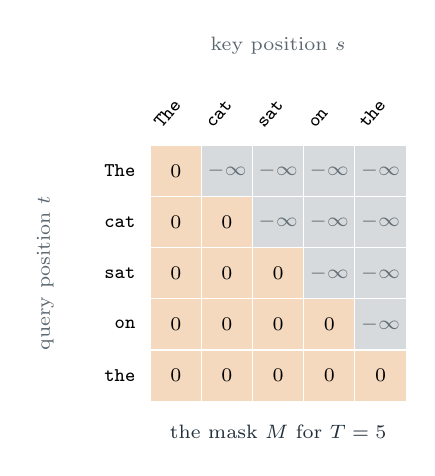
\begin{tikzpicture}[x=6.5mm,y=6.5mm]
  \foreach \r in {1,...,5} \foreach \c in {1,...,5} {
    \ifnum\c>\r
      \node[cell,minimum size=6.5mm,draw=white,fill=cInk!18,text=cInk!70] at (\c,-\r) {$-\infty$};
    \else
      \node[cell,minimum size=6.5mm,draw=white,fill=cAtt!30] at (\c,-\r) {$0$};
    \fi
  }
  \foreach \i/\w in {1/The,2/cat,3/sat,4/on,5/the} {
    \node[font=\scriptsize\ttfamily,anchor=east] at (0.4,-\i) {\w};
    \node[font=\scriptsize\ttfamily,rotate=50,anchor=south west] at (\i-0.25,-0.45) {\w};
  }
  \node[note,rotate=90] at (-1.55,-3) {query position $t$};
  \node[note] at (3,1.45) {key position $s$};
  \node[note,text=cInk] at (3,-6.1) {the mask $M$ for $T=5$};
\end{tikzpicture}

\vspace{0.5mm}
{\scriptsize\color{cTok}Row $t$ may look at columns $1..t$ only.}
\end{columns}
\end{frame}

% ======================================================================= 8
\begin{frame}{Stage 3 \textbullet{} Self-attention: a worked example ($T=3$, $d_k=2$)}
\small
Three tokens, one head. Follow the formula left to right (run \texttt{python walkthrough.py} to reproduce):
\vspace{-1mm}
{\footnotesize
\[
\underbrace{\begin{bmatrix}1&0\\0&2\\2&1\end{bmatrix}}_{Q}
\underbrace{\begin{bmatrix}1&0&2\\1&2&0\end{bmatrix}}_{K^{\T}}\!\frac{1}{\sqrt2}
=\underbrace{\begin{bmatrix}0.71&0&1.41\\1.41&2.83&0\\2.12&1.41&2.83\end{bmatrix}}_{\text{scores }S}
\;\xrightarrow{\;+M\;}\;
\begin{bmatrix}0.71&\color{cTok}-\infty&\color{cTok}-\infty\\1.41&2.83&\color{cTok}-\infty\\2.12&1.41&2.83\end{bmatrix}
\;\xrightarrow{\;\text{row softmax}\;}\;
\underbrace{\begin{bmatrix}1&0&0\\ \color{cAtt}0.196&\color{cAtt}0.804&0\\0.284&0.140&0.576\end{bmatrix}}_{\text{weights }A}
\]}
\vspace{-2mm}
\begin{columns}[T,onlytextwidth]
\column{0.52\textwidth}
{\footnotesize
\[
\text{output}=AV=A\underbrace{\begin{bmatrix}1&0\\0&1\\1&1\end{bmatrix}}_{V}
=\begin{bmatrix}1&0\\ \color{cAtt}0.196&\color{cAtt}0.804\\0.860&0.716\end{bmatrix}
\]}
\textbf{Row 2 by hand.} Scores $(1.41,\;2.83)$:
\[
  \frac{e^{1.41}}{e^{1.41}+e^{2.83}}=\frac{4.11}{4.11+16.92}=0.196,\qquad 1-0.196=0.804 .
\]
Its output is $0.196\,v_1+0.804\,v_2=(0.196,\,0.804)$.
\column{0.45\textwidth}
\begin{block}{Read the result}
\footnotesize
\begin{itemize}
  \item \textbf{Row 1} can only see itself: weight 1, output $=v_1$.
  \item \textbf{Row 2} prefers token 2 (higher score) but keeps 20\% of token 1.
  \item \textbf{Row 3} sees all three; its output mixes all values.
  \item Every row of $A$ is a probability distribution, and $A$ is lower-triangular.
        Both are checked in \texttt{test\_model.py}.
\end{itemize}
\end{block}
\end{columns}
\end{frame}

% ======================================================================= 9
\begin{frame}{Stage 3 \textbullet{} Multi-head attention: several lookups in parallel}
\begin{columns}[T,onlytextwidth]
\column{0.53\textwidth}
\small
One head gives one weighted average per position. Language needs several relations at once
(the subject, the previous word, the matching quote\dots), so run $h$ heads side by side, each
with its own $W_Q^{i},W_K^{i},W_V^{i}\in\R^{d\times d_k}$, $d_k=d/h$:
\[
  \MHA(X)=\bigl[\Attn_1(X)\,\Vert\,\cdots\,\Vert\,\Attn_h(X)\bigr]\,W_O ,
  \qquad W_O\in\R^{d\times d}.
\]
\centering
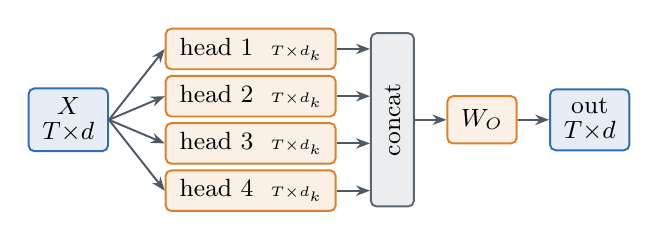
\begin{tikzpicture}[node distance=3mm,font=\scriptsize]
  \node[stage=cEmb,minimum height=6mm] (x) {$X$\\[-2pt]$T{\times}d$};
  \foreach \i/\y in {1/9,2/3,3/-3,4/-9}
    \node[stage=cAtt,minimum height=4.6mm,minimum width=16mm] (h\i) at ($(x.east)+(18mm,\y mm)$) {head \i\ \ {\tiny$T{\times}d_k$}};
  \node[stage=cTok,minimum height=22mm,minimum width=5mm] (cat) at ($(x.east)+(36mm,0)$) {\rotatebox{90}{concat}};
  \node[stage=cAtt,right=4mm of cat,minimum height=6mm] (wo) {$W_O$};
  \node[stage=cEmb,right=4mm of wo,minimum height=6mm] (o) {out\\[-2pt]$T{\times}d$};
  \foreach \i in {1,...,4} { \draw[flow] (x.east) -- (h\i.west); \draw[flow] (h\i.east) -- (h\i.east -| cat.west); }
  \draw[flow] (cat)--(wo); \draw[flow] (wo)--(o);
\end{tikzpicture}

\raggedright\vspace{1mm}
\begin{itemize}
  \item Splitting $d$ into $h$ pieces keeps the cost of one wide head.
  \item $W_O$ mixes the heads back into the shared $d$-dimensional space.
  \item In code this is one reshape: $(B,T,d)\to(B,h,T,d_k)$.
\end{itemize}
\column{0.44\textwidth}
\centering
{\small\textbf{Two heads of our trained model, block 1}}

\vspace{1mm}
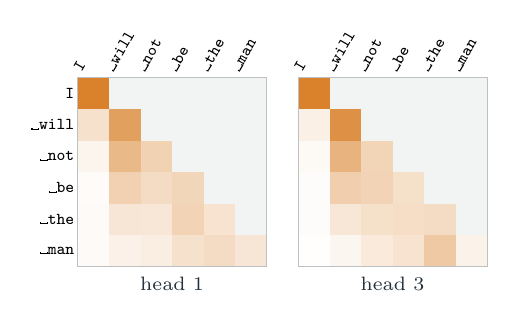
\begin{tikzpicture}[x=1mm,y=1mm,font=\ttfamily\fontsize{5.6}{6}\selectfont]
\fill[cAtt!100!white] (0.0,0.0) rectangle ++(4.0,-4.0);
\fill[cInk!6] (4.0,0.0) rectangle ++(4.0,-4.0);
\fill[cInk!6] (8.0,0.0) rectangle ++(4.0,-4.0);
\fill[cInk!6] (12.0,0.0) rectangle ++(4.0,-4.0);
\fill[cInk!6] (16.0,0.0) rectangle ++(4.0,-4.0);
\fill[cInk!6] (20.0,0.0) rectangle ++(4.0,-4.0);
\fill[cAtt!24!white] (0.0,-4.0) rectangle ++(4.0,-4.0);
\fill[cAtt!76!white] (4.0,-4.0) rectangle ++(4.0,-4.0);
\fill[cInk!6] (8.0,-4.0) rectangle ++(4.0,-4.0);
\fill[cInk!6] (12.0,-4.0) rectangle ++(4.0,-4.0);
\fill[cInk!6] (16.0,-4.0) rectangle ++(4.0,-4.0);
\fill[cInk!6] (20.0,-4.0) rectangle ++(4.0,-4.0);
\fill[cAtt!8!white] (0.0,-8.0) rectangle ++(4.0,-4.0);
\fill[cAtt!56!white] (4.0,-8.0) rectangle ++(4.0,-4.0);
\fill[cAtt!36!white] (8.0,-8.0) rectangle ++(4.0,-4.0);
\fill[cInk!6] (12.0,-8.0) rectangle ++(4.0,-4.0);
\fill[cInk!6] (16.0,-8.0) rectangle ++(4.0,-4.0);
\fill[cInk!6] (20.0,-8.0) rectangle ++(4.0,-4.0);
\fill[cAtt!3!white] (0.0,-12.0) rectangle ++(4.0,-4.0);
\fill[cAtt!37!white] (4.0,-12.0) rectangle ++(4.0,-4.0);
\fill[cAtt!28!white] (8.0,-12.0) rectangle ++(4.0,-4.0);
\fill[cAtt!33!white] (12.0,-12.0) rectangle ++(4.0,-4.0);
\fill[cInk!6] (16.0,-12.0) rectangle ++(4.0,-4.0);
\fill[cInk!6] (20.0,-12.0) rectangle ++(4.0,-4.0);
\fill[cAtt!4!white] (0.0,-16.0) rectangle ++(4.0,-4.0);
\fill[cAtt!20!white] (4.0,-16.0) rectangle ++(4.0,-4.0);
\fill[cAtt!19!white] (8.0,-16.0) rectangle ++(4.0,-4.0);
\fill[cAtt!35!white] (12.0,-16.0) rectangle ++(4.0,-4.0);
\fill[cAtt!22!white] (16.0,-16.0) rectangle ++(4.0,-4.0);
\fill[cInk!6] (20.0,-16.0) rectangle ++(4.0,-4.0);
\fill[cAtt!4!white] (0.0,-20.0) rectangle ++(4.0,-4.0);
\fill[cAtt!11!white] (4.0,-20.0) rectangle ++(4.0,-4.0);
\fill[cAtt!14!white] (8.0,-20.0) rectangle ++(4.0,-4.0);
\fill[cAtt!24!white] (12.0,-20.0) rectangle ++(4.0,-4.0);
\fill[cAtt!28!white] (16.0,-20.0) rectangle ++(4.0,-4.0);
\fill[cAtt!20!white] (20.0,-20.0) rectangle ++(4.0,-4.0);
\draw[cInk!30,line width=0.2pt] (0.0,0) rectangle ++(24.0,-24.0);
\node[rotate=60,anchor=south west,inner sep=0.5pt] at (0.6,0.3) {I};
\node[rotate=60,anchor=south west,inner sep=0.5pt] at (4.6,0.3) {\textvisiblespace will};
\node[rotate=60,anchor=south west,inner sep=0.5pt] at (8.6,0.3) {\textvisiblespace not};
\node[rotate=60,anchor=south west,inner sep=0.5pt] at (12.6,0.3) {\textvisiblespace be};
\node[rotate=60,anchor=south west,inner sep=0.5pt] at (16.6,0.3) {\textvisiblespace the};
\node[rotate=60,anchor=south west,inner sep=0.5pt] at (20.6,0.3) {\textvisiblespace man};
\node[anchor=east,inner sep=1pt] at (0,-2.0) {I};
\node[anchor=east,inner sep=1pt] at (0,-6.0) {\textvisiblespace will};
\node[anchor=east,inner sep=1pt] at (0,-10.0) {\textvisiblespace not};
\node[anchor=east,inner sep=1pt] at (0,-14.0) {\textvisiblespace be};
\node[anchor=east,inner sep=1pt] at (0,-18.0) {\textvisiblespace the};
\node[anchor=east,inner sep=1pt] at (0,-22.0) {\textvisiblespace man};
\node[font=\scriptsize,text=cInk] at (12.0,-26.2) {head 1};
\fill[cAtt!100!white] (28.0,0.0) rectangle ++(4.0,-4.0);
\fill[cInk!6] (32.0,0.0) rectangle ++(4.0,-4.0);
\fill[cInk!6] (36.0,0.0) rectangle ++(4.0,-4.0);
\fill[cInk!6] (40.0,0.0) rectangle ++(4.0,-4.0);
\fill[cInk!6] (44.0,0.0) rectangle ++(4.0,-4.0);
\fill[cInk!6] (48.0,0.0) rectangle ++(4.0,-4.0);
\fill[cAtt!12!white] (28.0,-4.0) rectangle ++(4.0,-4.0);
\fill[cAtt!88!white] (32.0,-4.0) rectangle ++(4.0,-4.0);
\fill[cInk!6] (36.0,-4.0) rectangle ++(4.0,-4.0);
\fill[cInk!6] (40.0,-4.0) rectangle ++(4.0,-4.0);
\fill[cInk!6] (44.0,-4.0) rectangle ++(4.0,-4.0);
\fill[cInk!6] (48.0,-4.0) rectangle ++(4.0,-4.0);
\fill[cAtt!5!white] (28.0,-8.0) rectangle ++(4.0,-4.0);
\fill[cAtt!61!white] (32.0,-8.0) rectangle ++(4.0,-4.0);
\fill[cAtt!34!white] (36.0,-8.0) rectangle ++(4.0,-4.0);
\fill[cInk!6] (40.0,-8.0) rectangle ++(4.0,-4.0);
\fill[cInk!6] (44.0,-8.0) rectangle ++(4.0,-4.0);
\fill[cInk!6] (48.0,-8.0) rectangle ++(4.0,-4.0);
\fill[cAtt!2!white] (28.0,-12.0) rectangle ++(4.0,-4.0);
\fill[cAtt!38!white] (32.0,-12.0) rectangle ++(4.0,-4.0);
\fill[cAtt!35!white] (36.0,-12.0) rectangle ++(4.0,-4.0);
\fill[cAtt!25!white] (40.0,-12.0) rectangle ++(4.0,-4.0);
\fill[cInk!6] (44.0,-12.0) rectangle ++(4.0,-4.0);
\fill[cInk!6] (48.0,-12.0) rectangle ++(4.0,-4.0);
\fill[cAtt!2!white] (28.0,-16.0) rectangle ++(4.0,-4.0);
\fill[cAtt!19!white] (32.0,-16.0) rectangle ++(4.0,-4.0);
\fill[cAtt!25!white] (36.0,-16.0) rectangle ++(4.0,-4.0);
\fill[cAtt!27!white] (40.0,-16.0) rectangle ++(4.0,-4.0);
\fill[cAtt!28!white] (44.0,-16.0) rectangle ++(4.0,-4.0);
\fill[cInk!6] (48.0,-16.0) rectangle ++(4.0,-4.0);
\fill[cAtt!1!white] (28.0,-20.0) rectangle ++(4.0,-4.0);
\fill[cAtt!7!white] (32.0,-20.0) rectangle ++(4.0,-4.0);
\fill[cAtt!17!white] (36.0,-20.0) rectangle ++(4.0,-4.0);
\fill[cAtt!22!white] (40.0,-20.0) rectangle ++(4.0,-4.0);
\fill[cAtt!43!white] (44.0,-20.0) rectangle ++(4.0,-4.0);
\fill[cAtt!10!white] (48.0,-20.0) rectangle ++(4.0,-4.0);
\draw[cInk!30,line width=0.2pt] (28.0,0) rectangle ++(24.0,-24.0);
\node[rotate=60,anchor=south west,inner sep=0.5pt] at (28.6,0.3) {I};
\node[rotate=60,anchor=south west,inner sep=0.5pt] at (32.6,0.3) {\textvisiblespace will};
\node[rotate=60,anchor=south west,inner sep=0.5pt] at (36.6,0.3) {\textvisiblespace not};
\node[rotate=60,anchor=south west,inner sep=0.5pt] at (40.6,0.3) {\textvisiblespace be};
\node[rotate=60,anchor=south west,inner sep=0.5pt] at (44.6,0.3) {\textvisiblespace the};
\node[rotate=60,anchor=south west,inner sep=0.5pt] at (48.6,0.3) {\textvisiblespace man};
\node[font=\scriptsize,text=cInk] at (40.0,-26.2) {head 3};
\end{tikzpicture}


\vspace{0.5mm}
{\scriptsize\color{cTok}Row = query token, column = key token; darker = larger weight.
Measured from \texttt{out/ckpt.pt}; the upper triangle is exactly zero.}
\end{columns}
\end{frame}

% ====================================================================== 10
\begin{frame}{Stage 4 \textbullet{} Feed-forward network and the activation function}
\begin{columns}[T,onlytextwidth]
\column{0.52\textwidth}
\small
Attention \emph{moves} information between positions. The feed-forward network (FFN)
\emph{transforms} it, at every position independently, with the same weights:
\[
  \FFN(x)=\GELU(xW_1+b_1)\,W_2+b_2,
\]
\[
  W_1\in\R^{d\times 4d},\qquad W_2\in\R^{4d\times d}.
\]
\begin{itemize}
  \item \textbf{Expand, bend, project}: $d\to4d\to d$. The wide hidden layer is where
        most parameters live: $\approx\!\tfrac23$ of each block.
  \item \key{Why a nonlinearity?} Without it, $W_1W_2$ is one matrix and the whole stack
        of layers could only compute linear functions of its input.
  \item \key{Which one?} $\GELU(x)=x\,\Phi(x)$, with $\Phi$ the standard normal CDF \cite{8}:
        a smooth ReLU with nonzero gradient for $x<0$. Used by GPT-2 and BERT.
        Recent models often use the related SiLU inside a gated FFN (SwiGLU \cite{18}).
\end{itemize}
\column{0.45\textwidth}
\centering
\begin{tikzpicture}
\begin{axis}[width=7.4cm,height=4.9cm,axis lines=left,xmin=-4,xmax=3.2,ymin=-0.5,ymax=3.1,grid=major,grid style={cInk!10},
  xtick={-4,-3,...,3},ytick={0,1,2,3},tick label style={font=\tiny},
  legend style={font=\scriptsize,draw=none,fill=none,at={(0.03,0.97)},anchor=north west},
  legend cell align=left,every axis plot/.append style={line width=1pt,no marks}]
  \addplot[cTok,dashed] table[x=x,y=relu]{generated/act.dat}; \addlegendentry{ReLU $\max(0,x)$}
  \addplot[cFfn] table[x=x,y=gelu]{generated/act.dat}; \addlegendentry{GELU $x\Phi(x)$}
  \addplot[cOut,densely dotted] table[x=x,y=silu]{generated/act.dat}; \addlegendentry{SiLU $x\sigma(x)$}
\end{axis}
\end{tikzpicture}

\vspace{0.5mm}
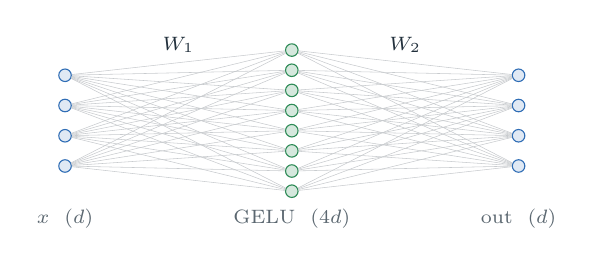
\begin{tikzpicture}[x=3.2mm,y=3.2mm]
  \foreach \i in {0,...,3}  \node[circle,draw=cEmb,fill=cEmb!15,inner sep=1.6pt] (a\i) at (0,\i*1.2-1.8) {};
  \foreach \j in {0,...,7}  \node[circle,draw=cFfn,fill=cFfn!20,inner sep=1.6pt] (b\j) at (9,\j*0.8-2.8) {};
  \foreach \i in {0,...,3}  \node[circle,draw=cEmb,fill=cEmb!15,inner sep=1.6pt] (c\i) at (18,\i*1.2-1.8) {};
  \foreach \i in {0,...,3} \foreach \j in {0,...,7} { \draw[cInk!25,line width=0.2pt] (a\i)--(b\j); \draw[cInk!25,line width=0.2pt] (b\j)--(c\i); }
  \node[note,below] at (0,-3.1) {$x$ \ ($d$)};
  \node[note,below] at (9,-3.1) {GELU \ ($4d$)};
  \node[note,below] at (18,-3.1) {out \ ($d$)};
  \node[note,above,text=cInk] at (4.5,2.3) {$W_1$}; \node[note,above,text=cInk] at (13.5,2.3) {$W_2$};
\end{tikzpicture}
\end{columns}
\end{frame}

% ====================================================================== 11
\begin{frame}{Stage 5 \textbullet{} Residual connections and LayerNorm: one block}
\centering
\vspace{2mm}
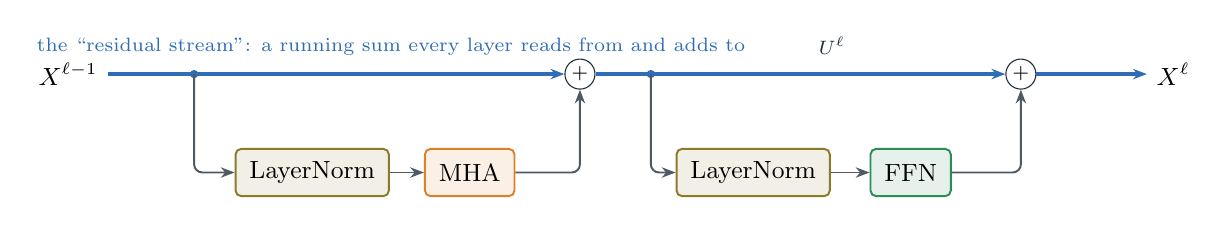
\begin{tikzpicture}[font=\small]
  \coordinate (in) at (0,0);
  \node[circle,draw=cInk,inner sep=1pt,font=\scriptsize] (p1) at (6.0,0) {$+$};
  \node[circle,draw=cInk,inner sep=1pt,font=\scriptsize] (p2) at (11.6,0) {$+$};
  \coordinate (out) at (13.2,0);
  \node[stage=cNrm,minimum height=6mm] (n1) at (2.6,-1.25) {LayerNorm};
  \node[stage=cAtt,minimum height=6mm] (at) at (4.6,-1.25) {MHA};
  \node[stage=cNrm,minimum height=6mm] (n2) at (8.2,-1.25) {LayerNorm};
  \node[stage=cFfn,minimum height=6mm] (ff) at (10.2,-1.25) {FFN};
  \draw[flow,line width=1.6pt,cEmb] (in) -- (p1); \draw[flow,line width=1.6pt,cEmb] (p1) -- (p2);
  \draw[flow,line width=1.6pt,cEmb] (p2) -- (out);
  \fill[cEmb] (1.1,0) circle (1.5pt); \fill[cEmb] (6.9,0) circle (1.5pt);
  \draw[flow,rounded corners=3pt] (1.1,0) |- (n1); \draw[flow] (n1)--(at); \draw[flow,rounded corners=3pt] (at) -| (p1);
  \draw[flow,rounded corners=3pt] (6.9,0) |- (n2); \draw[flow] (n2)--(ff); \draw[flow,rounded corners=3pt] (ff) -| (p2);
  \node[left,font=\small] at (in) {$X^{\ell-1}$}; \node[right,font=\small] at (out) {$X^{\ell}$};
  \node[note,above,text=cEmb] at (3.6,0.12) {the ``residual stream'': a running sum every layer reads from and adds to};
  \node[note,above,text=cInk] at (9.2,0.12) {$U^{\ell}$};
\end{tikzpicture}

\vspace{-1mm}
\[
  U^{\ell}=X^{\ell-1}+\MHA\bigl(\LN(X^{\ell-1})\bigr),\qquad
  X^{\ell}=U^{\ell}+\FFN\bigl(\LN(U^{\ell})\bigr)
\]
\vspace{-3mm}
\begin{columns}[T,onlytextwidth]
\column{0.48\textwidth}
\begin{block}{Residual connection \cite{7}}
\footnotesize
Each sublayer computes an \emph{update} that is added to its input.
\begin{itemize}
  \item The $+$ passes gradients straight through, so even the first block gets a clean
        training signal in a deep stack.
  \item At initialisation a block is close to the identity, a safe starting point.
\end{itemize}
\end{block}
\column{0.48\textwidth}
\begin{block}{Layer normalisation \cite{6}}
\footnotesize
Rescale each token's vector to mean 0, variance 1, then apply a learned gain and bias:
\[
  \LN(x)=\gamma\odot\frac{x-\mu(x)}{\sqrt{\sigma^2(x)+\epsilon}}+\beta,\qquad \gamma,\beta\in\R^{d}.
\]
Example: $\LN([2,4,6,8])=[-1.34,-0.45,0.45,1.34]$.
\end{block}
\end{columns}
\vspace{0.5mm}
{\footnotesize \key{Pre-LN} (shown; GPT-2 and later) normalises the \emph{input} of each sublayer and keeps the
stream itself untouched. The original transformer normalised after the addition; pre-LN trains more stably \cite{13}.}
\end{frame}

% ====================================================================== 12
\begin{frame}{The whole model on one slide}
\begin{columns}[T,onlytextwidth]
\column{0.60\textwidth}
\small
\textbf{Forward pass}, for token ids $x_{1:T}$:
\vspace{-1.5mm}
\begin{align*}
X^{0} &= E[x_{1:T}] + P_{1:T} && \text{\color{cEmb}embed}\\
U^{\ell} &= X^{\ell-1}+\MHA^{\ell}\bigl(\LN(X^{\ell-1})\bigr) && \text{\color{cAtt}communicate}\\
X^{\ell} &= U^{\ell}+\FFN^{\ell}\bigl(\LN(U^{\ell})\bigr),\quad \ell=1..L && \text{\color{cFfn}compute}\\
Z &= \LN(X^{L})\,E^{\T} && \text{\color{cOut}unembed}\\
p_\theta(\,\cdot\mid x_{\le t}) &= \softmax(Z_t) && \text{\color{cOut}predict}
\end{align*}
\vspace{-5mm}

\textbf{with the pieces}
\vspace{-1.5mm}
\begin{align*}
\Attn_i(X) &= \softmax\!\Bigl(\frac{(XW_Q^i)(XW_K^i)^{\T}}{\sqrt{d_k}}+M\Bigr)XW_V^i\\
\MHA(X) &= \bigl[\Attn_1(X)\,\Vert\cdots\Vert\,\Attn_h(X)\bigr]W_O\\
\FFN(X) &= \GELU(XW_1+b_1)\,W_2+b_2\qquad
\LN(x) = \gamma\odot\tfrac{x-\mu(x)}{\sigma(x)}+\beta
\end{align*}
\vspace{-5mm}

\textbf{Training} chooses $\theta=\{E,P,W^{\ell}_{\bullet},b^{\ell}_{\bullet},\gamma^{\ell}_{\bullet},\beta^{\ell}_{\bullet}\}$ to minimise
\ $\displaystyle\mathcal L(\theta) = -\frac1T\sum_{t=1}^{T}\log p_\theta\bigl(x_{t+1}\mid x_{\le t}\bigr)$
\column{0.37\textwidth}
\footnotesize
\textbf{Where the 875{,}264 parameters are}\\[1.5mm]
\renewcommand{\arraystretch}{1.15}
\begin{tabular}{@{}lrr@{}}
\toprule
component & formula & count\\
\midrule
$E$ (tokens) & $Vd$ & 65{,}536\\
$P$ (positions) & $T_{\max}d$ & 16{,}384\\
\midrule
attention & $4d^2+4d$ & 66{,}048\\
FFN & $8d^2+5d$ & 131{,}712\\
2 LayerNorms & $4d$ & 512\\
\textbf{one block} & & 198{,}272\\
$\times\,L=4$ & & 793{,}088\\
\midrule
final LayerNorm & $2d$ & 256\\
unembedding & tied to $E$ & 0\\
\bottomrule
\end{tabular}

\vspace{2mm}
Every operation is a matrix product, an addition, a normalisation, or an
element-wise function: all differentiable, so one call to backpropagation gives
$\nabla_\theta\mathcal L$.

\vspace{1mm}
A fuller formal treatment: \cite{15}.
\end{columns}
\end{frame}

% ====================================================================== 13
\begin{frame}{Stage 6 \textbullet{} From vectors back to tokens: unembedding and softmax}
\begin{columns}[T,onlytextwidth]
\column{0.51\textwidth}
\small
The final row $h_t=\LN(x^L_t)\in\R^d$ summarises the context. Score every vocabulary entry
with a dot product:
\[
  z = h_t\,E^{\T}\in\R^{V},\qquad z_j=h_t\cdot e_j .
\]
\begin{itemize}
  \item $z$ are the \key{logits}: token $j$ scores high when its embedding $e_j$ points the
        same way as $h_t$.
  \item \key{Weight tying} \cite{12}: reuse the embedding table $E$ as the output matrix. Fewer
        parameters, one shared meaning space.
\end{itemize}
\textbf{Softmax} turns scores into probabilities:
\[
  p_j=\softmax(z/\tau)_j=\frac{e^{z_j/\tau}}{\sum_{i=1}^{V}e^{z_i/\tau}}
\]
\begin{itemize}
  \item Positive, sums to 1, preserves order.
  \item Adding a constant to all $z_j$ changes nothing: only \emph{differences} matter.
  \item \key{Temperature} $\tau$: $\tau\to0$ picks the argmax; $\tau\to\infty$ is uniform.
\end{itemize}
\column{0.46\textwidth}
\centering
{\small ``The cat sat on the \rule{6mm}{0.4pt}'' \ logits $z=(2,\,1,\,0.5,\,0,\,-1)$}

\vspace{1mm}
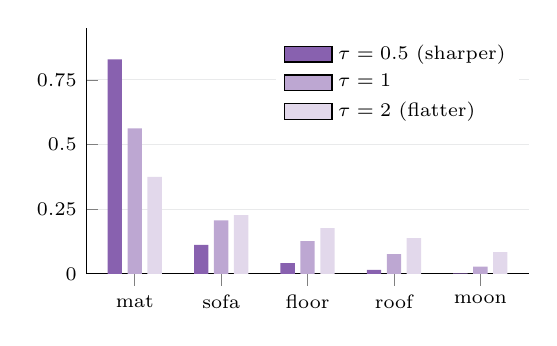
\begin{tikzpicture}
\begin{axis}[ybar,width=7.2cm,height=4.7cm,bar width=5.2pt,ymin=0,ymax=0.95,
  symbolic x coords={mat,sofa,floor,roof,moon},xtick=data,
  tick label style={font=\scriptsize},ytick={0,0.25,0.5,0.75},
  axis lines*=left,ymajorgrids,grid style={cInk!10},enlarge x limits=0.14,
  area legend,legend style={font=\scriptsize,draw=none,at={(0.98,0.98)},anchor=north east},legend cell align=left]
  \addplot[fill=cOut!90,draw=none] coordinates {(mat,0.829)(sofa,0.112)(floor,0.041)(roof,0.015)(moon,0.002)};
  \addplot[fill=cOut!50,draw=none] coordinates {(mat,0.563)(sofa,0.207)(floor,0.126)(roof,0.076)(moon,0.028)};
  \addplot[fill=cOut!22,draw=none] coordinates {(mat,0.375)(sofa,0.227)(floor,0.177)(roof,0.138)(moon,0.084)};
  \legend{$\tau=0.5$ (sharper),$\tau=1$,$\tau=2$ (flatter)}
\end{axis}
\end{tikzpicture}

\vspace{0.5mm}
{\footnotesize
\begin{tabular}{@{}lccccc@{}}
\toprule
 & mat & sofa & floor & roof & moon\\
\midrule
$\tau=0.5$ & .829 & .112 & .041 & .015 & .002\\
$\tau=1$ & .563 & .207 & .126 & .076 & .028\\
$\tau=2$ & .375 & .227 & .177 & .138 & .084\\
\bottomrule
\end{tabular}}
\end{columns}
\end{frame}

% ====================================================================== 14
\begin{frame}{Stage 7 \textbullet{} Generating text: choose a token, append, repeat}
\begin{columns}[T,onlytextwidth]
\column{0.44\textwidth}
\small
\begin{block}{The generation loop}
\begin{enumerate}\footnotesize
  \item Run the model on the tokens so far (at most the last $T_{\max}$).
  \item Take the logits of the \textbf{last} position only.
  \item Turn them into a distribution and \textbf{pick one token}.
  \item Append it. Go to 1.
\end{enumerate}
\end{block}
\centering
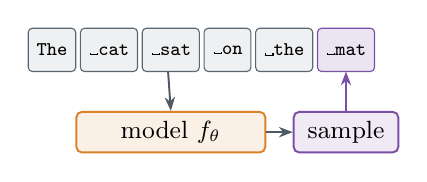
\begin{tikzpicture}[node distance=2.5mm,font=\scriptsize]
  \node[tokbox,font=\ttfamily\scriptsize] (a) {The};
  \node[tokbox,font=\ttfamily\scriptsize,right=0.6mm of a] (b) {\vsp cat};
  \node[tokbox,font=\ttfamily\scriptsize,right=0.6mm of b] (c) {\vsp sat};
  \node[tokbox,font=\ttfamily\scriptsize,right=0.6mm of c] (d) {\vsp on};
  \node[tokbox,font=\ttfamily\scriptsize,right=0.6mm of d] (e) {\vsp the};
  \node[tokbox,font=\ttfamily\scriptsize,right=0.6mm of e,draw=cOut,fill=cOut!15] (f) {\vsp mat};
  \node[stage=cAtt,minimum height=5mm,minimum width=24mm,below=5mm of c.south] (m) {model $f_\theta$};
  \node[stage=cOut,minimum height=5mm] (s) at (f |- m) {sample};
  \draw[flow] ($(a.south)!0.5!(e.south)$) -- (m.north);
  \draw[flow] (m)--(s);
  \draw[flow,cOut] (s.north) -- (f.south);
\end{tikzpicture}

\raggedright\vspace{1.5mm}
{\footnotesize The model is deterministic; all randomness enters at step 3. Production systems
cache each layer's keys and values so that a step costs one new row, not a full re-run.}
\column{0.53\textwidth}
\small
\textbf{Step 3: decoding strategies} on $p=(.563,\,.207,\,.126,\,.076,\,.028)$

\vspace{1mm}
{\footnotesize
\renewcommand{\arraystretch}{1.25}
\begin{tabular}{@{}p{18mm}>{\raggedright}p{36mm}>{\raggedright\arraybackslash}p{28mm}@{}}
\toprule
strategy & rule & result here\\
\midrule
\textbf{Greedy} & take $\arg\max_j p_j$ & always ``mat''\\
\textbf{Temperature} & sample from $\softmax(z/\tau)$ & $\tau{=}0.5$: mat 83\%\\
\textbf{Top-$k$} & keep the $k$ most likely, renormalise, sample & $k{=}2$:\ (.731, .269)\\
\textbf{Top-$p$} \cite{14} & keep the smallest set with total mass $\ge p$, renormalise, sample
   & $p{=}0.9$: drops ``moon''\\
\bottomrule
\end{tabular}}

\vspace{1.5mm}
\begin{itemize}\footnotesize
  \item Greedy is repeatable but tends to loop and repeat itself \cite{14}.
  \item Pure sampling ($\tau=1$) is diverse, but the long tail of unlikely tokens occasionally
        derails the text.
  \item Top-$k$ and top-$p$ cut the tail and then sample: the usual compromise.
        Top-$p$ adapts: few candidates when the model is sure, many when it is not.
\end{itemize}
{\footnotesize Top-$p$ check: cumulative mass $(.563,\,.770,\,.896,\,.972,\,1)$ first reaches $0.9$ at the 4th token.}
\end{columns}
\end{frame}

% ====================================================================== 15
\begin{frame}{Training \textbullet{} The objective: make the true next token likely}
\begin{columns}[T,onlytextwidth]
\column{0.50\textwidth}
\small
Training data is just text. Slide a window over it; the \textbf{target is the input shifted
by one token}:

\vspace{1mm}
\centering
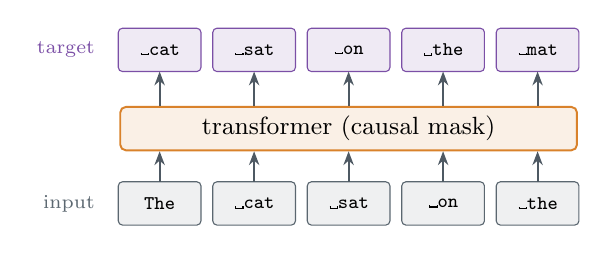
\begin{tikzpicture}[font=\scriptsize]
  \foreach \i/\w in {0/The,1/\vsp cat,2/\vsp sat,3/\vsp on,4/\vsp the}
    \node[tokbox,font=\ttfamily\scriptsize,minimum width=10.5mm] (i\i) at (\i*1.2,0) {\w};
  \foreach \i/\w in {0/\vsp cat,1/\vsp sat,2/\vsp on,3/\vsp the,4/\vsp mat}
    \node[tokbox,font=\ttfamily\scriptsize,minimum width=10.5mm,draw=cOut,fill=cOut!12] (o\i) at (\i*1.2,1.95) {\w};
  \node[stage=cAtt,minimum width=58mm,minimum height=5mm] (m) at (2.4,0.95) {transformer (causal mask)};
  \foreach \i in {0,...,4} { \draw[flow] (i\i.north) -- (i\i.north |- m.south); \draw[flow] (o\i.south |- m.north) -- (o\i.south); }
  \node[note,anchor=east] at (-0.7,0) {input}; \node[note,anchor=east,text=cOut] at (-0.7,1.95) {target};
\end{tikzpicture}

\raggedright\vspace{1mm}
Because of the mask, one sequence of length $T$ gives $T$ training examples in a single pass.

\vspace{1mm}
\textbf{Cross-entropy loss} (average negative log-likelihood):
\[
  \mathcal L(\theta)=-\frac{1}{T}\sum_{t=1}^{T}\log p_\theta\bigl(x_{t+1}\mid x_{\le t}\bigr)
\]
Assign probability 1 to the truth: loss 0. Assign it $0.207$: loss $-\ln 0.207=1.57$.
\column{0.47\textwidth}
\small
\begin{block}{The gradient is remarkably simple}
\footnotesize
For logits $z$, probabilities $p=\softmax(z)$ and one-hot target $y$:
\[
  \frac{\partial\mathcal L}{\partial z}=p-y .
\]
Push the correct logit up by $1-p_y$, push every other logit down by its own probability.
Backpropagation carries this signal to every weight.
\end{block}
{\footnotesize Example (target ``sofa''):
$p-y=(.563,\;{-.793},\;.126,\;.076,\;.028)$; confirmed against finite differences in
\texttt{walkthrough.py}.}

\vspace{1.5mm}
\begin{block}{Two sanity numbers}
\footnotesize
\begin{itemize}
  \item An untrained model guesses uniformly, so its loss should be $\ln V=\ln 512=6.24$.
        Ours started at 6.26.
  \item \textbf{Perplexity} $=e^{\mathcal L}$: the effective number of equally likely
        choices the model is hesitating between.
\end{itemize}
\end{block}
\end{columns}
\end{frame}

% ====================================================================== 16
\begin{frame}{Training \textbullet{} The optimizer: AdamW with warmup and cosine decay}
\begin{columns}[T,onlytextwidth]
\column{0.50\textwidth}
\small
Plain gradient descent is $\theta\leftarrow\theta-\eta\,g$ with $g=\nabla_\theta\mathcal L$ on a random
mini-batch. Transformers are trained with \key{AdamW} \cite{9,10}, which keeps two running averages
per parameter:
\vspace{-1mm}
\begin{align*}
 m_t &= \beta_1 m_{t-1}+(1-\beta_1)\,g_t && \text{mean of gradients}\\
 v_t &= \beta_2 v_{t-1}+(1-\beta_2)\,g_t^{2} && \text{mean of squares}\\
 \hat m_t &= \frac{m_t}{1-\beta_1^{t}},\quad \hat v_t=\frac{v_t}{1-\beta_2^{t}} && \text{bias correction}\\
 \theta_t &= \theta_{t-1}-\eta_t\Bigl(\frac{\hat m_t}{\sqrt{\hat v_t}+\epsilon}+\lambda\,\theta_{t-1}\Bigr)
\end{align*}
\vspace{-3mm}
\begin{itemize}\footnotesize
  \item \textbf{Momentum} ($m$) smooths noisy gradients.
  \item \textbf{Per-parameter scaling} ($\sqrt{v}$): each step is about $\eta$ in size whatever the
        gradient's scale. On step 1 it is exactly $\pm\eta$.
  \item \textbf{Decoupled weight decay} ($\lambda$): shrink weight matrices a little every step
        to regularise; not applied to biases or LayerNorm gains.
\end{itemize}
\column{0.47\textwidth}
\centering
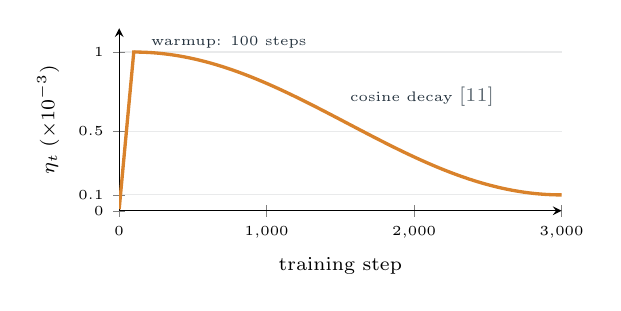
\begin{tikzpicture}
\begin{axis}[width=7.2cm,height=3.9cm,xmin=0,xmax=3000,ymin=0,ymax=1.15,
  xlabel={training step},ylabel={$\eta_t\;(\times10^{-3})$},
  label style={font=\scriptsize},tick label style={font=\tiny},
  xtick={0,1000,2000,3000},ytick={0,0.1,0.5,1},scaled x ticks=false,
  axis lines=left,ymajorgrids,grid style={cInk!10}]
  \addplot[cAtt,line width=1.2pt,domain=0:100,samples=2] {(x+1)/100};
  \addplot[cAtt,line width=1.2pt,domain=100:3000,samples=80] {0.1+0.45*(1+cos(180*(x-100)/2900))};
  \node[font=\tiny,anchor=west,text=cInk] at (axis cs:150,1.06) {warmup: 100 steps};
  \node[font=\tiny,anchor=west,text=cInk] at (axis cs:1500,0.72) {cosine decay \cite{11}};
\end{axis}
\end{tikzpicture}

\raggedright
{\footnotesize
\textbf{Warmup}: early on $v_t$ is a poor estimate and the weights are random, so start with small
steps. \textbf{Decay}: finish with small steps to settle into a minimum.
\textbf{Gradient clipping} \cite{16}: if $\lVert g\rVert_2>1$, rescale $g$ to norm 1 so one bad batch
cannot wreck the weights.}

\vspace{1.5mm}
{\footnotesize
\begin{tabular}{@{}llll@{}}
\toprule
\multicolumn{4}{@{}l}{\textbf{Settings in} \texttt{train.py}}\\
\midrule
peak $\eta$ & $10^{-3}$ & $\beta_1,\beta_2$ & $0.9,\ 0.95$\\
final $\eta$ & $10^{-4}$ & $\lambda$ & $0.1$\\
batch $\times$ $T$ & $32\times128$ & clip norm & $1.0$\\
\bottomrule
\end{tabular}}
\end{columns}
\end{frame}

% ====================================================================== 17
\begin{frame}[fragile]{Code \textbullet{} The model: each equation is a line of PyTorch (\texttt{model.py})}
\vspace{-1mm}
\lstinputlisting[style=py,linerange={35-36,51-58,60-62,65,74-75,78,88-91,94,123,127-131}]{../model.py}
\vspace{-1mm}
{\scriptsize\color{cTok}Lines included verbatim from \texttt{model.py} (constructors omitted). Compare with slides 7, 9, 10, 11 and 12.}
\end{frame}

% ====================================================================== 18
\begin{frame}[fragile]{Code \textbullet{} The training harness (\texttt{train.py})}
\vspace{-1mm}
\lstinputlisting[style=py,linerange={62-67,70-75,139,156-163}]{../train.py}
\vspace{-0.5mm}
{\footnotesize
\texttt{python train.py} trains the tokenizer, encodes the corpus (90/10 train/validation split), runs the
loop above (evaluation and checkpointing lines omitted), logs to \texttt{out/log.csv}, saves the best checkpoint by validation loss, and prints a sample.
Every hyperparameter is a flag: \texttt{-{}-n\_layer 6 -{}-n\_embd 384 -{}-block\_size 256} gives a GPU-sized model.}
\end{frame}

% ====================================================================== 19
\begin{frame}[fragile]{Results \textbullet{} What the harness produces}
\begin{columns}[T,onlytextwidth]
\column{0.44\textwidth}
\centering
\begin{tikzpicture}
\begin{axis}[width=6.9cm,height=4.6cm,xmin=0,xmax=3000,ymin=2.5,ymax=6.5,
  xlabel={training step},ylabel={loss (nats/token)},
  label style={font=\scriptsize},tick label style={font=\tiny},scaled x ticks=false,
  axis lines=left,ymajorgrids,grid style={cInk!10},
  legend style={font=\scriptsize,draw=none,at={(0.97,0.97)},anchor=north east},legend cell align=left]
  \addplot[cEmb,line width=1.1pt,mark=*,mark size=1pt] table[x=step,y=train_loss,col sep=comma]{generated/log.csv};
  \addplot[cAtt,line width=1.1pt,mark=square*,mark size=1pt] table[x=step,y=val_loss,col sep=comma]{generated/log.csv};
  \addplot[cTok,dashed,domain=0:3000,samples=2] {6.238};
  \legend{train,validation,$\ln V$}
\end{axis}
\end{tikzpicture}

\vspace{-1mm}
\raggedright
{\footnotesize
\textbf{\resSteps{} steps in \resMinutes{} minutes on 2 CPU cores.} Validation loss falls from
\resInit{} ($\approx\ln V$) to \resVal{} (train \resTrain): perplexity \resPpl, down from 512.
The train--validation gap is the model starting to memorise its 1\,MB corpus.
}
\column{0.53\textwidth}
\small
\textbf{Sample} (prompt: newline; $\tau=0.8$, top-$k=50$)
\lstinputlisting[style=py,language={},basicstyle=\ttfamily\fontsize{6.6}{8}\selectfont]{generated/sample.txt}
\vspace{-1mm}
{\footnotesize Shakespeare-shaped, not Shakespeare: with under a million parameters the model has learned
spelling, speaker labels and line structure, but little meaning. Scale $d$, $L$, data and compute, and the
same code becomes a real LLM.}

\vspace{1.5mm}
\begin{block}{Try it}
\footnotesize
\begin{itemize}
  \item \texttt{python test\_model.py}: initial loss $\approx\ln V$, causality, overfit one batch.
  \item \texttt{python walkthrough.py}: every worked number in these slides.
  \item Exercises: remove the mask and watch validation loss; set $h=1$; swap GELU for ReLU;
        train with \texttt{-{}-tokenizer char}.
\end{itemize}
\end{block}
\end{columns}
\end{frame}

% ====================================================================== 20
\begin{frame}{References}
\fontsize{6.4}{7.9}\selectfont
\begin{columns}[T,onlytextwidth]
\column{0.49\textwidth}
\begin{enumerate}[{[1]}]\setlength{\itemsep}{0.6pt}
\item Vaswani et al. \emph{Attention Is All You Need.} NeurIPS 2017. arXiv:1706.03762
\item Radford et al. \emph{Improving Language Understanding by Generative Pre-Training.} OpenAI, 2018. (GPT)
\item Radford et al. \emph{Language Models are Unsupervised Multitask Learners.} OpenAI, 2019. (GPT-2)
\item Sennrich, Haddow, Birch. \emph{Neural Machine Translation of Rare Words with Subword Units.} ACL 2016. arXiv:1508.07909
\item Bahdanau, Cho, Bengio. \emph{Neural Machine Translation by Jointly Learning to Align and Translate.} ICLR 2015. arXiv:1409.0473
\item Ba, Kiros, Hinton. \emph{Layer Normalization.} 2016. arXiv:1607.06450
\item He, Zhang, Ren, Sun. \emph{Deep Residual Learning for Image Recognition.} CVPR 2016. arXiv:1512.03385
\item Hendrycks, Gimpel. \emph{Gaussian Error Linear Units (GELUs).} 2016. arXiv:1606.08415
\item Kingma, Ba. \emph{Adam: A Method for Stochastic Optimization.} ICLR 2015. arXiv:1412.6980
\item Loshchilov, Hutter. \emph{Decoupled Weight Decay Regularization.} ICLR 2019. arXiv:1711.05101
\end{enumerate}
\column{0.49\textwidth}
\begin{enumerate}[{[1]}]\setlength{\itemsep}{0.6pt}
\setcounter{enumi}{10}
\item Loshchilov, Hutter. \emph{SGDR: Stochastic Gradient Descent with Warm Restarts.} ICLR 2017. arXiv:1608.03983
\item Press, Wolf. \emph{Using the Output Embedding to Improve Language Models.} EACL 2017. arXiv:1608.05859
\item Xiong et al. \emph{On Layer Normalization in the Transformer Architecture.} ICML 2020. arXiv:2002.04745
\item Holtzman et al. \emph{The Curious Case of Neural Text Degeneration.} ICLR 2020. arXiv:1904.09751
\item Phuong, Hutter. \emph{Formal Algorithms for Transformers.} 2022. arXiv:2207.09238
\item Pascanu, Mikolov, Bengio. \emph{On the Difficulty of Training Recurrent Neural Networks.} ICML 2013. arXiv:1211.5063
\item Su et al. \emph{RoFormer: Enhanced Transformer with Rotary Position Embedding.} 2021. arXiv:2104.09864
\item Shazeer. \emph{GLU Variants Improve Transformer.} 2020. arXiv:2002.05202
\item Karpathy. \emph{nanoGPT} (code) and the Tiny Shakespeare corpus (\emph{char-rnn}). github.com/karpathy
\end{enumerate}

\vspace{2mm}
{\fontsize{7}{8.6}\selectfont\color{cInk}
\textbf{Further reading.} [15] gives complete pseudocode for every transformer variant.
[1] is the original (encoder--decoder, post-LN, sinusoidal positions); [3] is the decoder-only,
pre-LN, GELU design implemented here.

\vspace{1mm}
\textbf{Reproducibility.} All numbers on slides 4--5, 8 and 13--16 are printed by
\texttt{walkthrough.py}; slides 9 and 19 are generated from the training run by
\texttt{make\_figures.py}.}
\end{columns}
\end{frame}

\end{document}
